\documentclass{article}
\usepackage{graphicx}
\usepackage{listings}
\usepackage{color}
\usepackage{float}
\usepackage{tikz}
\usetikzlibrary{shapes, arrows, positioning}

\title{Practical Work 3: MPI File Transfer}
\author{Nguyen Thanh Dat \\ Student ID: 23BI14091}
\date{}

\begin{document}

\maketitle

\section{Introduction}
The goal of this practical work is to implement a file transfer system using the **Message Passing Interface (MPI)** standard. 
Unlike the previous client-server models (TCP and RPC) where distinct programs connected over a network socket, this system uses a **Single Program, Multiple Data (SPMD)** model where multiple processes communicate via messages.

\section{MPI Implementation Choice}
For this implementation, I chose **OpenMPI** running on **Kali Linux**.

\subsection{Justification}
\begin{itemize}
    \item \textbf{Native Support:} Kali Linux (Debian-based) provides native support for OpenMPI via the APT package manager, ensuring a stable environment without the driver compatibility issues often found on Windows.
    \item \textbf{Environment Integration:} As a security-focused distribution, Kali allows for seamless network process management, making it an ideal environment for testing distributed protocols.
    \item \textbf{Library:} I used \texttt{mpi4py} because it provides Pythonic bindings for the MPI standard, allowing for high-level object serialization (pickling) while maintaining the underlying performance of the C-based OpenMPI drivers.
\end{itemize}

\section{Service Design}
The system consists of two processes launched simultaneously by the MPI executor. They are distinguished by their \textbf{Rank}.

\begin{figure}[H]
    \centering
    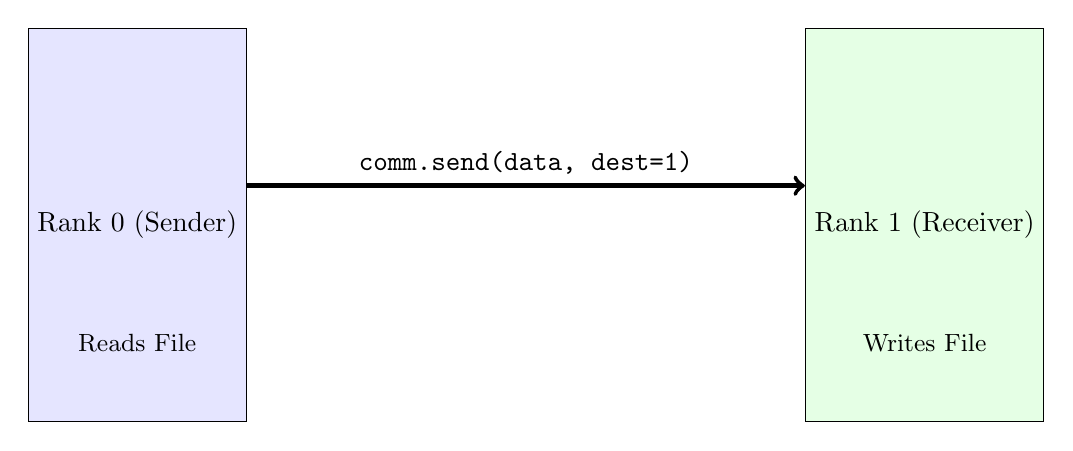
\begin{tikzpicture}[node distance=10cm, auto]

        \node (rank0) [draw, rectangle, minimum height=5cm, fill=blue!10] {Rank 0 (Sender)};
        \node (rank1) [draw, rectangle, minimum height=5cm, fill=green!10, right of=rank0] {Rank 1 (Receiver)};

        \draw[->, ultra thick] ([yshift=0.5cm]rank0.east) -- node[above] {\texttt{comm.send(data, dest=1)}} ([yshift=0.5cm]rank1.west);

        \node[below of=rank0, node distance=1.5cm] {\small Reads File};
        \node[below of=rank1, node distance=1.5cm] {\small Writes File};
    \end{tikzpicture}
    \caption{MPI Point-to-Point Communication Design}
    \label{fig:mpi_design}
\end{figure}

\section{Implementation}
The logic is contained within a single file, \texttt{transfer.py}. The execution path splits based on the process rank.

\begin{lstlisting}[language=Python, basicstyle=\small, breaklines=true, frame=single]
from mpi4py import MPI
import os

comm = MPI.COMM_WORLD
rank = comm.Get_rank()

if rank == 0:
    # SENDER LOGIC
    with open('test.jpg', 'rb') as f:
        file_data = f.read()
    
    # Package data into a dictionary
    data_package = {'filename': 'test.jpg', 'content': file_data}
    
    # Blocking send
    comm.send(data_package, dest=1, tag=0)
    print(f"Sent {len(file_data)} bytes to Rank 1.")

elif rank == 1:
    # RECEIVER LOGIC
    data = comm.recv(source=0, tag=0)
    
    with open('received_' + data['filename'], 'wb') as f:
        f.write(data['content'])
    print("File saved successfully.")
\end{lstlisting}

\section{Verification}
The following screenshot demonstrates the execution in the Kali Linux terminal. It shows Rank 0 successfully sending the bytes and Rank 1 confirming the save operation.

 \begin{figure}[H]
    \centering
    \includegraphics[width=0.9\textwidth]{proof.png}
    \caption{Successful MPI Execution on Kali Linux}
 \end{figure}

\end{document}